\documentclass{beamer}
\mode<presentation>
{
  \usetheme{Singapore}
  \setbeamercovered{transparent}
}

\usepackage[english]{babel}
\usepackage[utf8]{inputenc}
\usepackage{times}
\usepackage[T1]{fontenc}
\usepackage{algorithm2e}
\usepackage{algorithmic}
\usepackage{float}
\usepackage{amsmath}


\title[Short Paper Title] % (optional, use only with long paper titles)
{Social Graph Learning}

\author[Author, Another] % (optional, use only with lots of authors)
{Steve Poulson}

\institute[Universities of Somewhere and Elsewhere] % (optional, but mostly needed)
{Supervisor: Dell Zhang, Mark Levine}

\date[CFP 2003] % (optional, should be abbreviation of conference name)
{28 May 2013}
\subject{Theoretical Computer Science}
\pgfdeclareimage[height=1cm]{university-logo}{cisco.png}
%\logo{\pgfuseimage{university-logo}}

\AtBeginSubsection[]
{
  \begin{frame}<beamer>{Outline}
    \tableofcontents[currentsection,currentsubsection]
  \end{frame}
}

% If you wish to uncover everything in a step-wise fashion, uncomment
% the following command: 

%\beamerdefaultoverlayspecification{<+->}


\begin{document}

\begin{frame}
  \titlepage
\end{frame}

\begin{frame}
\frametitle{Types of social graphs}
\begin{table}[h!]
     \begin{center}
     \begin{tabular}[c]{ l  p{5cm}  p{5cm}  }
      Unipartite, Undirected e.g. LinkedIn & \includegraphics[width=1cm]{../my_papers/figs/graph.png} &
      \\
     \pause
      Unipartite, Directed e.g. Google Plus & \includegraphics[width=1cm]{../my_papers/figs/digraph.png} &
      \\
      \pause
      Bipartite, UnDirected e.g. Netflix & \includegraphics[width=1cm]{../my_papers/figs/bipartite.png} &
      \end{tabular}
      \end{center}
      \end{table}
\end{frame}

\begin{frame}{Sampling}
We need to get the data, we could sample a real graph
\\
  \begin{itemize}
	\item Breadth First
	\pause
	\item Depth First
	\pause
	\item Snowball
	\pause
	\item Forest Fire
  \end{itemize}
In practise we need to simulate the growth of the graph
\end{frame}

\begin{frame}{Algorithm}
\begin{algorithm}[H]
 \SetAlgoLined
 \KwData{Directed Graph A}
 \KwResult{Digraph B with n new vertices, m new edges}
 \While{not n vertices}
 {
 	pick random edge $(v_1,v_2)$ from A where $v_1$ $\in$ B \\
 	add $v_2$
 	add $(v_1,v_2)$ to graph B\\
 }
  \While{not m edges added}
  {
  	pick random edge $(v_1,v_2)$ from A where $v_1,v_2$ $\in$ B \\
 	add $(v_1,v_2)$ to graph B\\
  }
 \caption{Grow}
\end{algorithm}
\end{frame}

\begin{frame}{Karate Dataset grown to t=4, n=10}

\includegraphics[width=10cm]{../my_papers/figs/Amazon_4.png}
  
\end{frame}

\begin{frame}{Supervised learning problem}
Formally
  \begin{itemize}
	\item $ \mathbf{Y}\leftarrow \mathbf{A^{t+1} }- \mathbf{A^t} $ 
	\pause
	\item $ \min(L ( f(\phi(\mathbf{A^t})) , \mathbf{Y})))$
	\pause
  \end{itemize}
\end{frame}

\begin{frame}{Feature Function $\phi$}

Maps $\mathbf{A}_{i,j} \rightarrow (x_1 \dots x_n)$  

  \begin{itemize}
	\item Random Walk between nodes
	\pause
	\item Modularity
	\pause
	\item Jaccard Distance of neighbour list
	\pause
	\item Betweeness Centrality
  \end{itemize}
\end{frame}

\begin{frame}{Betweeness}
\includegraphics[width=10cm]{../my_papers/figs/Amazon_Centrality_9.png}
\end{frame}

\begin{frame}{Jaccard Distance}
\includegraphics[width=10cm]{../my_papers/figs/Amazon_jaccard_9.png}
\end{frame}

\begin{frame}{Shortest Path}
\includegraphics[width=10cm]{../my_papers/figs/Amazon_shortest_path_9.png}
\end{frame}

\begin{frame}{Local vs Global}

  \begin{itemize}
	\item Global features from a 1 million node graph unfeasible  
	\pause
	\item Power Law graphs scale invariant so local features should characterize graph 
	\pause
	\item Can use Hadoop Map calculates subset of local features, reduce assembles training set which classifier runs on 
  \end{itemize}
\end{frame}

\begin{frame}{Let's try it on a Kaggle competition}
  \begin{itemize}
  	\item Prototyped on sklearn / networkx
   	\item Hadoop cluster on AWS
   	\item Java: Weka / Hadoop / cern.colt.matrix / Jung
   	\item Random Forrest classifer beat rest
  \end{itemize}
\end{frame}

%\begin{frame}{MLE}
%	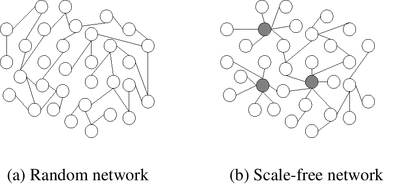
\includegraphics[width=5cm]{sf}
%   \begin{itemize}
%    	\item degree of vertex $X_i$
%   	\pause
%	\item Sample $n \log(\alpha) + n \alpha \log(m) - (\alpha+1) \sum_{i=1}^{n} \log(X_i)$
%	\pause
%	\item $\hat{m} = \min_{i} X_i$
%	\pause
%	\item $\frac{n}{\alpha} + n \log( \hat{m} ) - \sum_{i=1}^{n} \log(X_i) = 0$
%	\item $\hat{\alpha} = \frac{n}{\sum_{i=1}^{n} \log(X_i/\hat{m})}$.
%   \end{itemize}
%\end{frame}

\begin{frame}{Kaggle Evaluation}


\includegraphics[width=10cm]{kaggle}

  \begin{itemize}
	\item A bit of fun :)
	\pause
	\item  Mean Average Precision @ 10 = 0.71371
	\pause
	\item  Within 2\% of winner
  \end{itemize}
  
\end{frame}

\begin{frame}{Summary}
  \begin{itemize}
\item Power law Sampling gives a time varying dataset
	\pause
\item Random Forrest best
	\pause
\item Pretty good results

  \end{itemize}
\end{frame}

\begin{frame}{Future work}
  \begin{itemize}
\item Factorial Machines
\item Deep Learning
\item Sample real data Twitter / Google+
\item Bipartite Graphs
  \end{itemize}
\end{frame}



\end{document}


